\chapter{Keeping the user in control}\label{chap:control}

\graphicspath{{images/control/}}

\begin{framed}
	\textbf{Key points:}
	
	\begin{itemize}
		\item An experiment was designed to compared \gls{sparc} to another approach in \gls{iml}: \acrfull{irl} using feedback and partial guidance to teach a robot an action policy.
		\item Application domain is a replication of the world used in early studies on \acrshort{irl}.
		\item \gls{sparc} uses full control over the robot's action, implicit rewarding system and evaluation of intentions rather than actions.
		\item \gls{sparc} was combined with an algorithm from the \acrlong{rl} field.
		\item Results show that \gls{sparc} achieves a better performance, easier and faster than \acrshort{irl}.
	\end{itemize}
\end{framed}

Parts of the work presented in this chapter have been published verbatim in \cite{senft2017supervised} \footnote{Note about technical contribution in this chapter: the author reimplemented every part of the system manually in Qt.}. The final publication is available from Elsevier via \url{https://doi.org/10.1016/j.patrec.2017.03.015}.

\newpage
\section{Motivation}

Previous work in \gls{iml} has been shown that humans want to teach robots not only with feedback but also by communicating what the robot should do \citep{thomaz2008teachable}. However, in most of the research teaching agents a policy using human guidance, the teacher is given few or no control at all on the agent's action and has to observe the agent executing an undesired actions even when knowing that this action is incorrect. This chapter explores how these \gls{iml} approaches could be pushed further by applying the principles of \gls{sparc} defined in Chapter \ref{chap:sparc} and how it would influence the learning process, the agent performance and the user experience.

Additionally, the previous study explored how \gls{sparc} could be used with an algorithm from the \gls{sl} domains, to replicate a teacher's action policy, but some of the most promising features of \gls{iml} arise when combined with algorithm from the \gls{rl} field. As such this study uses an reinforcement learning algorithm to teach the robot.

The goal of this study is twofold: exploring how to apply \gls{sparc} to algorithms from \gls{rl} and comparing how this human control over the robot's actions impacts the learning. As such, it has been decided to compare an approach using \gls{sparc} to one offering less control but having been validated in previous studies: \acrfull{irl} \citep{thomaz2008teachable}. The testing environment of \gls{irl} have be reimplemented to stay as close as possible to the online version of the task.

\section{Scope of the study}

\subsection{Interactive Reinforcement Learning}

The \gls{irl} algorithms implements the principles presented in \cite{thomaz2008teachable}. In \gls{irl} the human teacher can provide positive or negative feedback on the last action executed by the robot. The robot combines this with environmental feedback into a reward which is used to update a Q-table: a table with a Q-values (the expected discounted reward) assigned to every state-action pair and used to select the next action. Three additions to the standard algorithm have been proposed and implemented by Thomaz and Breazeal and are used here as well: guidance, communication by the robot and an undo option \citep{thomaz2008teachable}. Teachers have two way to transmit information to the robot: the reward channel (to give a numerical on the last action) and the guidance channel (to direct attention toward parts of the state).

The guidance emerged from the results of a pilot study where participants assigned rewards to objects to indicate that the robot should do something with these objects. With the guidance, teachers can direct the attention of the robot toward certain item in the environment to indicate the robot that it should interact with them. This guidance behaviour offer partial control over the robot's actions and restricts the next action the robot is executing, but it cannot be used to set explicitly the robot behaviour. 

The robot also communicates its uncertainty by directing its gaze toward different items in the environment with equally high probability of being used next. The aim of this communication of uncertainty is to provide transparency about the robot's internal state, for example indicating when a guidance should be provided. 

Finally, after a negative reward, the robot tries to cancel the effect of the previous action (if possible), resulting in a undo behaviour. As shown in the original paper, these three additions improve the performance on the task.

\subsection{SPARC}

\gls{sparc} uses a single type of input similar to the guidance present in \gls{irl} but without using the reward channel. However with \gls{sparc}, the guidance channel controls directly the actions of the robot. The robot communicates every of its intentions (i.e the action it plans to execute next) to its teacher by looking to a part of the environment and the teacher can either not intervene, letting the robot execute the suggested action or step in and force the robot to execute an alternative action. This combination of suggestions and corrections gives the teacher full control over the actions executed by the robot. This also makes the rewards redundant: rather than requiring the human to explicitly provide rewards, a positive reward is directly assigned to each action executed by the robot as it has been either forced or passively approved by the teacher.

\subsection{Differences of approaches}

Unlike \gls{irl}, \gls{sparc} offers full control over the actions executed by the robot. \gls{sparc} changes the learning paradigm from learning from the human evaluation of actions' effects to learning from the human's expectation of these actions' effects and preferences. An expert in the task domain evaluates the appropriateness of actions before their execution and can guide the robot to act as they see correct. This implies that the robot does not to rely on observing negative effect of an action to learn that this action should be avoided, but rather what the best action is for each state. Even in a non-deterministic environment such as \gls{hri}, some actions can be expected to have a negative consequence. The human teacher can stop the robot from ever executing these actions, preventing the robot from causing harm to itself or its social or physical environment. 

Another noticeable difference is the way in which the robot communicates with the user: in \gls{irl}, the robot communicates its uncertainty about an action and with \gls{sparc} its intention to execute an action. It should also be noted that the quantity of information provided by the user to the robot is similar for both \gls{irl} and \gls{sparc}: in \gls{sparc} the user can offer the whole action space as commands to the robot, which removes the need for explicit rewards. While in \gls{irl}, the teacher can guide the robot toward a subset of the action space but has to manually provide feedbacks to evaluate the robot's decisions.

\subsection{Hypotheses}

Three hypotheses have been tested in the study:
\begin{enumerate}
	\item [H1] \textit{Effectiveness and efficiency with non-experts.} Compared to \gls{irl}, \gls{sparc} leads to higher performance, whilst being faster, requiring fewer inputs and less mental effort from the teacher and minimising the number of errors during the teaching phase when used by non-experts.
	\item [H2] \textit{Safety with experts.} \gls{sparc} can be used by experts to teach an action policy safely, quickly and efficiently, unlike other \gls{iml} methods lacking control.
	\item [H3] \textit{Control.} Teachers prefer a method in which they can have more control over the robot's actions.
\end{enumerate}
\section{Methodology}

The task used in this study is the same as \cite{thomaz2008teachable}: Sophie's kitchen, a simulated environment on a computer where a virtual robot has to learn how to bake a cake in a kitchen. As the source code was not available, the task was reimplemented to stay as close as possible to the description in the paper and the online version of the task\footnote{\url{http://www.cc.gatech.edu/~athomaz/sophie/WebsiteDeployment/}}.

The scenario is the following: a robot, Sophie, is in a kitchen with three different locations (shelf, table and oven) and five objects (flour, tray, eggs, spoon and bowl) as shown in Figure \ref{fig:control_initial}. Sophie has to learn how to bake a cake and the participant has to guide the robot through a sequence of steps while giving enough feedback so the robot learns a correct series of actions. As presented in Figure \ref{fig:control_states}, there are six crucial steps to achieve a successful result:

\begin{enumerate}
	\item Put the bowl on the table (Figure \ref{fig:control_bowl}).
	\item Add one ingredient to the bowl (flour or eggs).
	\item Add the second ingredient (Figure \ref{fig:control_ingredients}).
	\item Mix the ingredients with the spoon to obtain batter (Figure \ref{fig:control_batter}).
	\item Pour the batter in the tray (Figure \ref{fig:control_tray}).
	\item Put the tray in the oven (Figure \ref{fig:control_goal}).
\end{enumerate}

The environment is a deterministic Markov Decision Process, defined by a state, a set of actions (move left, move right, pick up, drop and use), a deterministic transition function and environmental reward function (+1 for success and -1 for failure and -0.04 for every other step to penalise long sequences). Different action policies can lead to success, but many actions end in a failure state, for example putting the spoon in the oven results in a failure. As argued by Thomaz and Breazeal, this environment provides a good setup to evaluate teaching methods to a robot due to the large number of possible states (more than 10,000), the presence of success and failure states and the sparse nature of the environmental reward function which increases the need for a teacher to aid the learning. More details on the environment are available in the original paper.

\subsection{Task}
\begin{figure}[ht]
	\centering
	\begin{subfigure}[b]{0.3\textwidth}
		\centering
		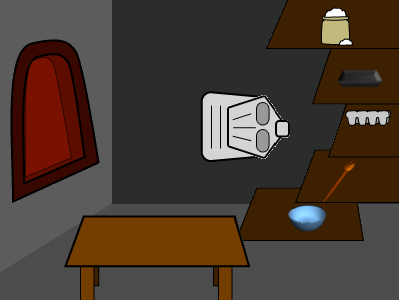
\includegraphics[width=\textwidth]{step0.png}
		\caption{Initial state}
		\label{fig:control_initial}
	\end{subfigure}
	\centering
	\begin{subfigure}[b]{0.3\textwidth}
		\centering
		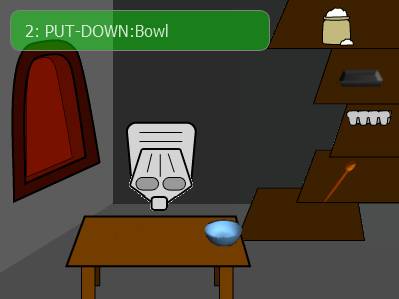
\includegraphics[width=\textwidth]{step1.png}
		\caption{Step 1}
		\label{fig:control_bowl}
	\end{subfigure}
	\centering
	\begin{subfigure}[b]{0.3\textwidth}
		\centering
		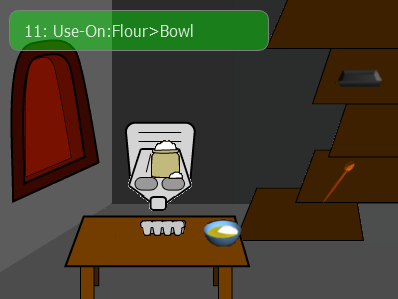
\includegraphics[width=\textwidth]{step3.png}
		\caption{Step 3}
		\label{fig:control_ingredients}
	\end{subfigure}
	
	
	\centering
	\begin{subfigure}[b]{0.3\textwidth}
		\centering
		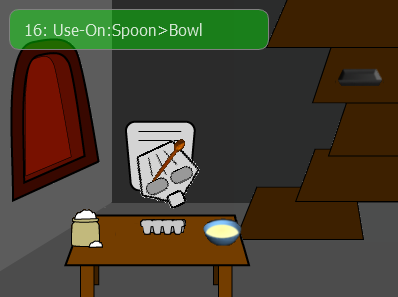
\includegraphics[width=\textwidth]{step4.png}
		\caption{Step 4}
		\label{fig:control_batter}
	\end{subfigure}
	\centering
	\begin{subfigure}[b]{0.3\textwidth}
		\centering
		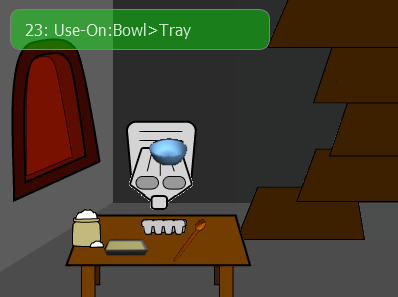
\includegraphics[width=\textwidth]{step5.png}
		\caption{Step 5}
		\label{fig:control_tray}
	\end{subfigure}
	\centering
	\begin{subfigure}[b]{0.3\textwidth}
		\centering
		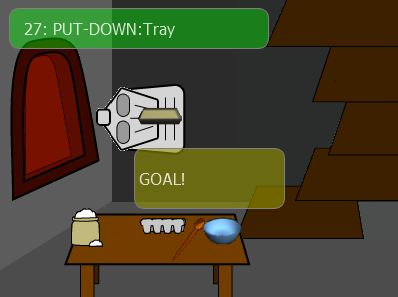
\includegraphics[width=\textwidth]{step6.png}
		\caption{Step 6}
		\label{fig:control_goal}
	\end{subfigure}
	
	\caption{Presentation of different steps in the environment. \ref{fig:control_initial} initial state, \ref{fig:control_bowl} step 1: the bowl on the table, \ref{fig:control_ingredients} step 3: both ingredients in the bowl, \ref{fig:control_batter} step 4: ingredients mixed to obtain batter, \ref{fig:control_tray} step 5: batter poured in the tray and \ref{fig:control_goal} step 6 (success): tray with batter put in the oven. (Step 2: one ingredient in the bowl has been omitted for clarity)}
	\label{fig:control_states}
\end{figure}

\subsection{Conditions}

Two conditions are compared for this study: \gls{irl} and \gls{sparc}. The underlying learning is strictly identical for both conditions, only the way to interact with it, how to provide it rewards changes: with \gls{irl} teachers have to explicitly provide rewards, while they are implicit with \gls{sparc}. 

The learning algorithm (see Algorithms \ref{algo:control_sparc} and \ref{algo:control_irl}) is a variation on Q-learning, without reward propagating\footnote{In Q learning the update function is $Q(s_{t},a_{t}) \leftarrow Q(s_{t},a_{t}) + \alpha (r_{t+1}+\gamma (\underset{a}{max} Q(s_{t+1},a))-Q(s_{t},a_{t}))$}. This guarantees that any learning by the robot is due to the teaching by the human, and as such provides a lower bound for the robot's performance. By using Q-learning, the performance of the robot would be higher.

\begin{minipage}[t]{0.5\textwidth}
	\vspace{0pt}  
	\begin{algorithm}[H]
		\caption{Algorithm used for SPARC}
		\label{algo:control_sparc}
		 \While{learning}{
		 	$a$ = action with the highest $Q[s,a]$
		 	
		 	look at object or location used with $a$
		 	
		 	\While{waiting for correction (2 seconds)}{
		 		\eIf{received command}{
		 			$a$ = received command
		 			
		 			reward, $r = 0.5$
		 		}{
		 		reward, $r = 0.25$
		 	}
		 }
		 execute $a$, and transition to $s'$
		 $r = r + r_{environment}$
		 
		 Learn: $Q(s_{t},a_{t}) \leftarrow Q(s_{t},a_{t}) + \alpha (r_{t+1}+\gamma (\underset{a}{max} Q(s_{t},a))-Q(s_{t},a_{t}))$
		}
	\end{algorithm}
\end{minipage}%
\begin{minipage}[t]{0.5\textwidth}
	\vspace{0pt}
	\begin{algorithm}[H]
		\caption{Algorithm used for IRL
			\vspace{0.2pt}}
		\label{algo:control_irl}
		\While{learning}{
			$a$ = action with the highest $Q[s,a]$
			
			indicate confusion if multiple $a$ with similar high $Q[s,a]$
			
			\While{waiting for guidance and reward on last action (2 seconds)}{
				\If{received command}{
					Try: $a$ = received command
				}
				\If{received reward $r'$}{
					$r = r + r'$				
				}
		}
		
		Learn: $Q(s_{t},a_{t}) \leftarrow Q(s_{t},a_{t}) + \alpha (r_{t+1}+\gamma (\underset{a}{max} Q(s_{t},a))-Q(s_{t},a_{t}))$
		execute $a$, and transition to $s'$
		$r = r_{environment}$
		
		\vspace{5.5pt}
	}
	\end{algorithm}
\end{minipage}
%CHange += and environmental r

\subsubsection{Interactive Reinforcement Learning}

We have implemented \gls{irl} following the principles presented in \cite{thomaz2008teachable}. The user can use the left click to display a slider providing rewards. The guidance is implemented by right-clicking on objects: it directs the robot's attention to the object if facing it (a click on objects in different locations has no effect). Following the guidance, the robot will execute the candidate action involving the object. The action space is not entirely covered by this guidance mechanism: for example, it does not cover moving from a location to another. This guidance if used correctly, limits the exploration for the current step to the part of the environment evaluated as more interesting by the user without preventing the robot to explore in further steps. The robot can communicate its uncertainty by looking at multiple objects having similarly high probability of being used. 

Some modifications were required to the original study due to the lack of implementation details in the original paper, one of them being the use of a purely greedy action selection instead of using softmax, due to the absence of parameters descriptions. The reliance on human rewards and guidance limits the importance of autonomous exploration, and thus, the greediness of the algorithm should assist the learning by preventing the robot to explore outside of the guided policy. Additionally, as the environment is deterministic and the algorithm is greedy, the concept of convergence is altered: once a trajectory has Q-Values high enough or a correct gradient of Q-Values on all state-action pairs, it will be reinforced automatically.

\subsubsection{SPARC}

\gls{sparc} uses the gaze of the robot toward objects or locations to indicate which action the robot is suggesting to the teacher. Similarly to the guidance in \gls{irl}, the teacher can use the right click of the mouse on objects to have the robot execute the action associated to this object in the current state and this has been extended to also cover locations. With \gls{sparc}, the command covers all the action space: at every time step, the teacher can specify, if desired, the next action executed by the robot. If an action is not corrected, a positive reward of 0.25 is automatically received (as it has the implicit approval from the teacher) and if the teacher selects another action, a reward of 0.5 is given to the correcting action (the corrected action is not rewarded). That way, actions actively selected are more reinforced and participants can still have give higher rewards when using \gls{irl}. This system allows for the use of reinforcement learning with implicit reward assignation, which simplifies the teaching interaction.


\subsection{Interaction protocol}

Participants are divided into two groups and interact first either with \gls{irl} or \gls{sparc} as shown in Figure \ref{fig:control_design}. Before interacting, participants complete a demographic questionnaire and receive a information sheet explaining the task (describing the environment and how to bake the cake) and one explaining the system they are interacting with. Then they interact for three sessions with the assigned system. Each session is composed of a training phase and a testing phase. The training phase is composed of as many teaching episodes as the participant desires, a teaching episode ends when a success or failure state has been reached which returns the environment to the initial state. In the same way as in the initial experiment by Thomaz and Breazeal, participants can decide to terminate the training phase whenever they desire by clicking on a button labelled `Sophie is ready', however it is also terminated after 25 minutes to impose an upper time limit to the study. After the end of a training phase, the robot runs a testing phase where the participant's inputs are disabled and which stops as soon as an ending state is reached or the participants decide to stop it (for example if the robot is stuck in a loop). This testing phase is used to evaluate the performance of the participants for this session. The interaction with a system consists of three repeated independent sessions with their own independent training and testing phases to observe how the interactions evolve as participants are getting used to the system.

After participants completed their three sessions with the first system, they are asked to interact for three more sessions with the other system. This way, every participant interacts three times with each system (\gls{irl} and \gls{sparc}) and the order of interaction is balanced. Additionally, participants have to complete post-interaction questionnaires distributed after the interaction with the first system and the second one and a final post-experiment questionnaire at the end of the experiment. All information sheets and questionnaires can be found online \footnote{\url{https://emmanuel-senft.github.io/experiment2.html}}.


This experimental design prevents the risk of having an ordering effect by having a symmetry between conditions. Both conditions having a identical experimental procedure only with the order of interaction varying.

\begin{figure}[t!]
	\centering
	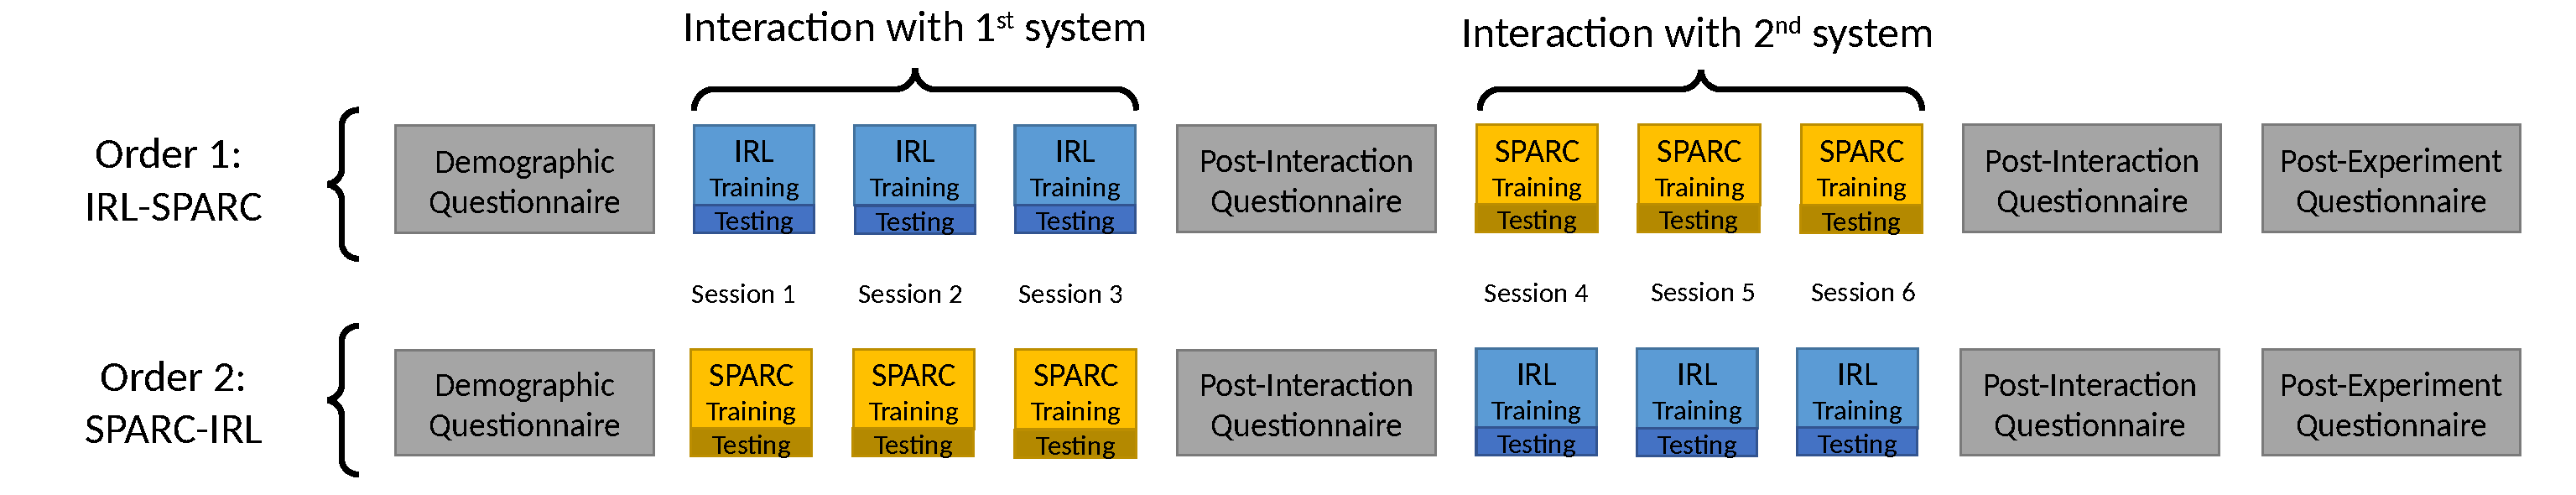
\includegraphics[width=1\textwidth]{fullDesign.pdf}
	\caption{Participants are divided into two groups. They first complete a demographic questionnaire, then interact for three independent sessions (with a training and a testing phase each) with a system (IRL or SPARC). After a first post-interaction questionnaire, participants interact for another three sessions with the other system before completing the second post-interaction questionnaire and a final post-experiment questionnaire.}
	\label{fig:control_design}
\end{figure}

\subsection{Participants}

A total of 40 participants have been recruited using a tool provided by the university to reach a mixed population of students and non-student members of the local community.  All participants gave written informed consent, and were told of the option to withdraw at any point. All participants received remuneration at the standard U.K. living wage rate, pro rata. Participants were distributed randomly between the groups whilst balancing gender and age (age \textit{M}=25.6, \textit{SD}=10.09; 24F/16M). Participants were mostly not knowledgeable in machine learning and robotics (average familiarity with machine learning \textit{M}=1.8, \textit{SD}=1.14; familiarity with social robots \textit{M}=1.45, \textit{SD}=0.75 - Likert scale ranging from 1 to 5).

In addition to naive non-expert users, an expert user (the author) interacted five times with each system following a strictly optimal strategy in both cases. These results from the expert are used to evaluate H2 and show the optimal characteristics of each system (\gls{irl} and \gls{sparc) when used by trained experts such as therapist in a context of assistive robotics.

\subsection{Metrics}

\subsubsection{Interaction Metrics}

We collected three metrics during the training phase: the number of times a participant reached a failure state while teaching, which can be related to the risks taken during the training and the teaching time (from 0 to 25 minutes) and the number of inputs provided during the training, which can be seen as the efforts invested in the teaching. The testing phase is a single run of the taught action policy ending as soon as the robot reaches an ending state (failure or success) or if stopped by the participants. We only use the performance achieved during this single test as evaluation of the success of training. As not all participants reached a success during the testing phase, we used the six key steps defined in subsection \ref{ssec:task} as a way to evaluate the performance ranging from 0 (no step has been completed) to 6 (the task was successfully completed) during this testing run: for example a testing where the robot puts both ingredients in the bowl but reaches a failure state before mixing them would have a performance of 3.

\subsubsection{Questionnaires}

The post-interaction and post-experiment questionnaires provide additional subjective information to compare with the objective results from the interaction data. Two principal metrics are gathered: the workload on participants and the perception of the robot. 

Workload is an important factor when teaching robots. As roboticists, our task is to make the teaching of robots as undemanding as possible, meaning that the workload for user should be minimal. Multiple definitions for workload exist and various measures can be found in the literature. Due to its widespread use in human factors research and clear definition and evaluation criteria, we used the NASA-Task Load Index (TLX) \citep{hart1988development}. We averaged the values from the 6 scales (mental, physical and temporal demand, performance, effort and frustration) to obtain a single workload value per participant for each interaction. So we have two measures for each participant, after interaction with the first system and after the interaction using the other system.

Finally, the perception of the robot has been evaluated in the post-interaction and post-experiment questionnaires using subjective questions (measured on a Likert scale), binary questions (which robot did you prefer interacting with) and open questions on preference and naturalness of the interaction. 

\section{Results}

\section{Discussion}

\section{Summary}

